\section{Results}

Results were obtained for an arbitrary maneuver. The initial state is neutral attitude: roll, pitch and yaw all equal to zero. The final state are the following roll, pitch and yaw angles (in that order):
\begin{equation}
\phi=-20^\circ \quad \theta=10^\circ \quad \psi=90^\circ
\end{equation}

We are particularly interested in two of the norms. The 2-norm and $\infty$-norm. The 2-norm shows the maneuver for the shortest path, it can be computed in real time using the approximation provided in section IIIc, and works as a reference solution. The $\infty$-norm uses three independent bounds, resembles more closely the limits of an attitude control system, and offers the possibility for unexplored more optimal solutions than those found by the 2-norm.

We start by discussing in detail the solution for the 2-norm solution. Figure \ref{fig:l2Maneuver} shows the main characteristics of the maneuver. Time-history is provided for the main parameters of interest: the states, attitude (in Euler angles) and angular velocity, the applied torques and the co-states that the determine the input. The co-states of the attitude are not represented since they do not offer any additional insight. The initial co-states for the maneuver are:
\begin{equation}
\lambda_{q_0} = [-0.0006 \quad 0.2474 \quad 0.0833 \quad -0.9532]^T \qquad
\lambda_{\omega_0} = [0.1583 \quad 0.0533 \quad -.6093]
\end{equation}

The total time used for the maneuver is $2.5596$ non-dimensional time units and the amplitude of total rotated angle is $1.6378$ radians. A closer look to the graphics reveals that our initial guess for the solution is indeed correct. The $\lambda_{\omega}$ behave linearly with time and being equal to 0 at exactly the half of the motion where the inputs reverse. The amplitude of these is set so that they are aligned with the eigenaxis of the rotation.

\begin{figure}[H]
	\centering
	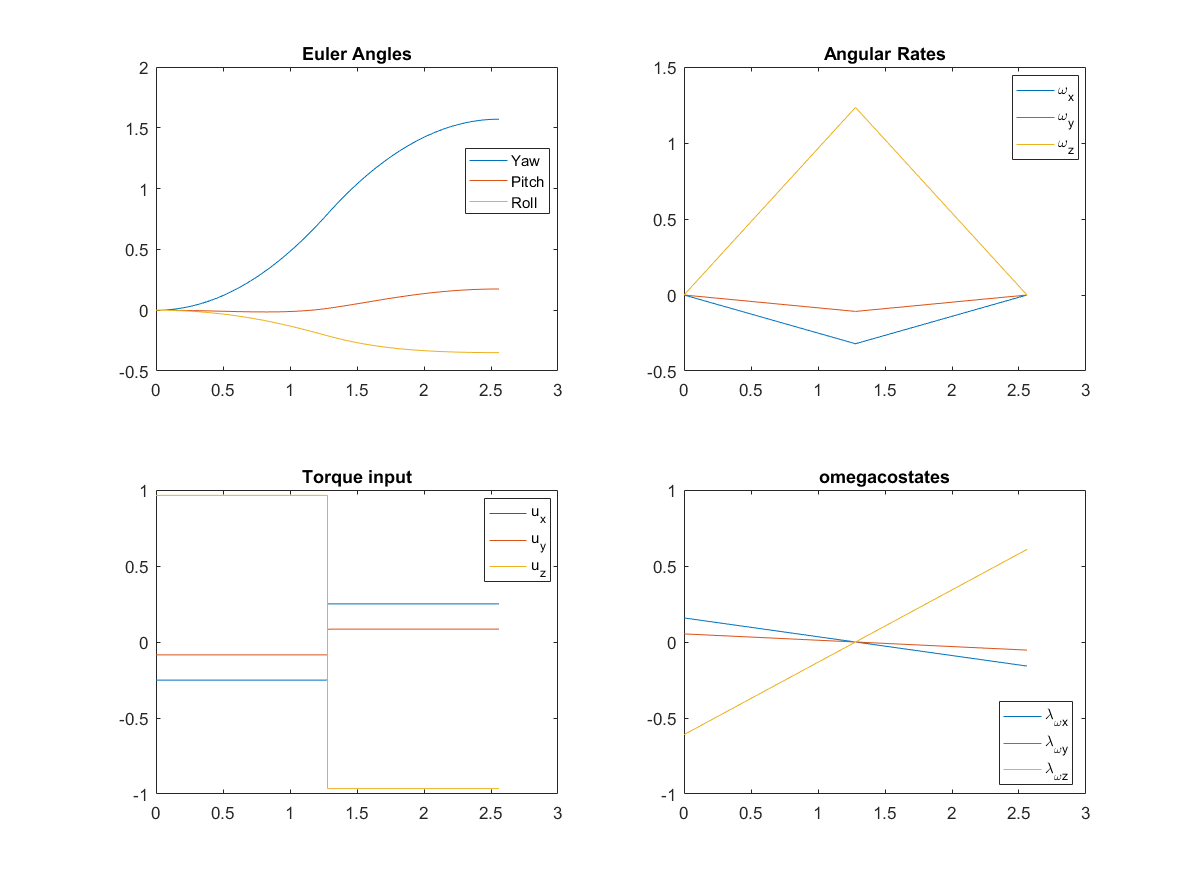
\includegraphics[height=12cm,keepaspectratio]{media/l2Maneuver.png}
	\caption{Solution, inputs and co-states for the switching function for the 2-norm optimal maneuver.}
	\label{fig:l2Maneuver}
\end{figure}

We now proceed to discuss the continuation process to the infinity norm. This was done by increasing the norm of the controller a about a 10 percent each iteration up to a norm of 20. Figure \ref{fig:lConvergence} shows some selected norms in the continuation process that show the evolution of the controller. As the norm of the controls increase the coupling between axes becomes more and more relaxed, for the $\infty$-norm they should be three independent controls bounds so the all three controls should lie on the $\pm1$ bound.

\begin{figure}[h]
	\centering
	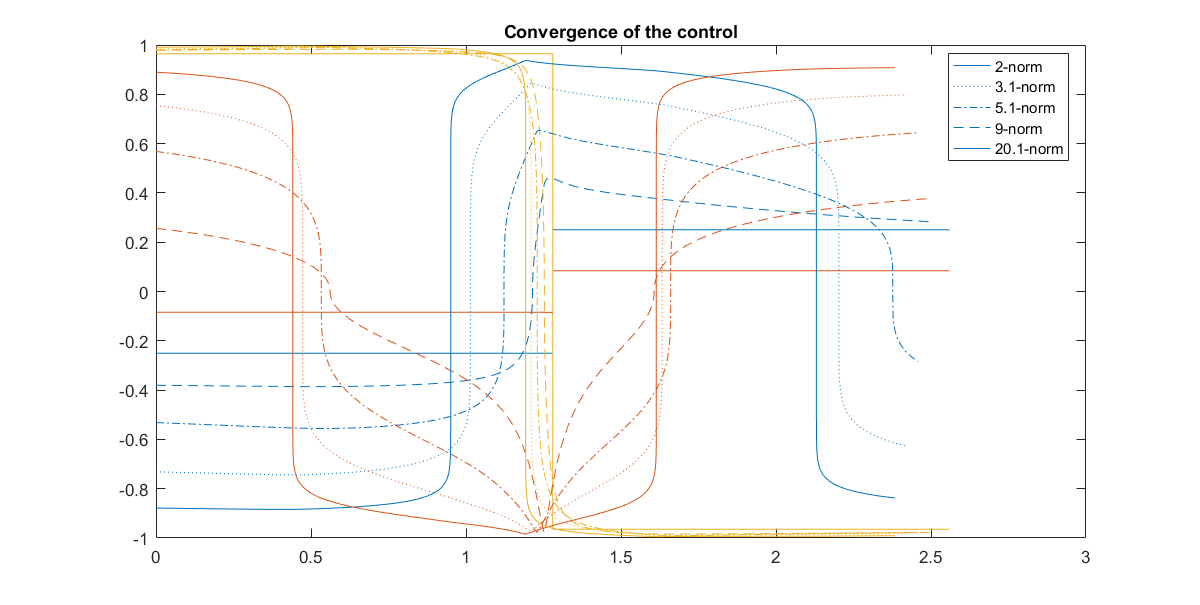
\includegraphics[height=8cm,keepaspectratio]{media/controlConvergence.png}
	\caption{Three axes controls for different norms ranging from to 2 to 20. As the norm increases the three controls become more and more decoupled. Reproduced from Bilimoria \cite{bilimoria1993time}.}
	\label{fig:lConvergence}
\end{figure}

Once the 20-norm controller is found, it is used as the starting solution for the $\infty$-norm controller implemented as in equation \ref{lInfinityControl}. The three controls become completely indepdent, the characteristics for the new control are plotted in figure \ref{fig:lInftyManeuver} in a similar fashion to those of the 2-norm control. The initial value for the co-states is:
\begin{equation}
\lambda_{q_0} = [-0.0405 \quad 0.0809 \quad -0.3818 \quad -0.9179]^T \qquad
\lambda_{\omega_0} = [0.0594 \quad -0.0751 \quad -.5617]
\end{equation}

\begin{figure}[H]
	\centering
	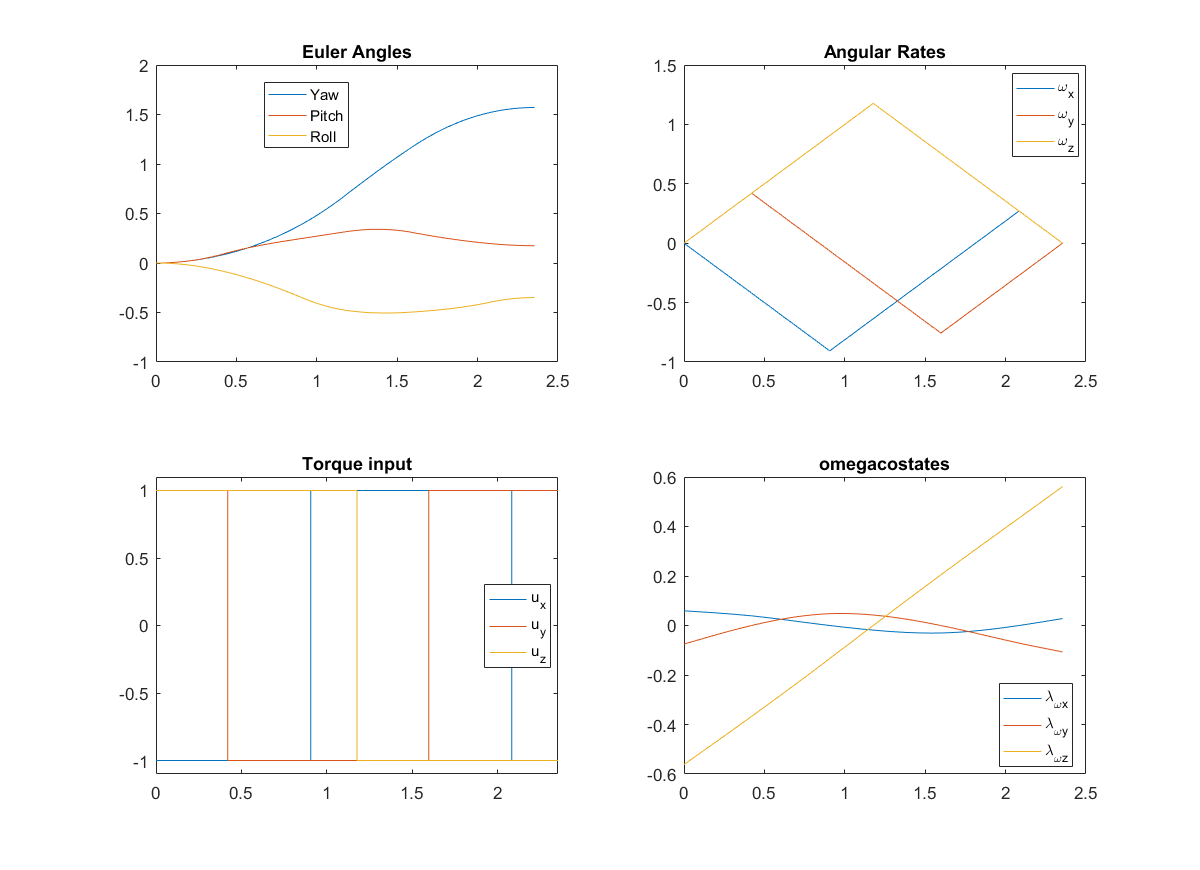
\includegraphics[height=12cm,keepaspectratio]{media/lInftyManeuver.png}
	\caption{Solution, inputs and costates for the switching function for the $\infty$-norm optimal maneuver.}
	\label{fig:lInftyManeuver}
\end{figure}

The maneuver time has decreased to $2.3540$. A decrease above 8\% in the maneuver time. The controls have the form of independent switching functions as it could be expected. This means that the angular velocity is also composed of linear intervals, this implies that the trajectory will be made up of analytically solvable intervals. A phase-space approach to the problem may offer additional insight on how to choose the switches and define a global strategy, but it will definitely be complex due the high number of states. The shape for the co-states of the switching function has become more complex. The results are coherent with those found by Bilimoria$\cite{bilimoria1993time}$ in terms of the shape of the switching function and the observed reduction in time.

Finally, in order to attempt to reproduce the results from Bilimoria \cite{bilimoria1993time}, a 180 degree in yaw maneuver was attempted. While this maneuver is the largest angle maneuver, and possibly will show the most benefit from our control strategy, the control to achieve it is not unique by the rotational symmetry of the problem. In this last piece of the results we attempted to obtain a control similar to the one he provides in Figure 6 in \cite{bilimoria1993time}. The angular velocity history obtained here is provided in figure \ref{fig:bilimoriaResults}. The results are identical, other than a mirrored $\omega_y$ due to the mentioned non-uniqueness of optimal control, the optimal time for the trajectory is 3.243 non-dimensional units same as the paper states.

\begin{figure}[H]
	\centering
	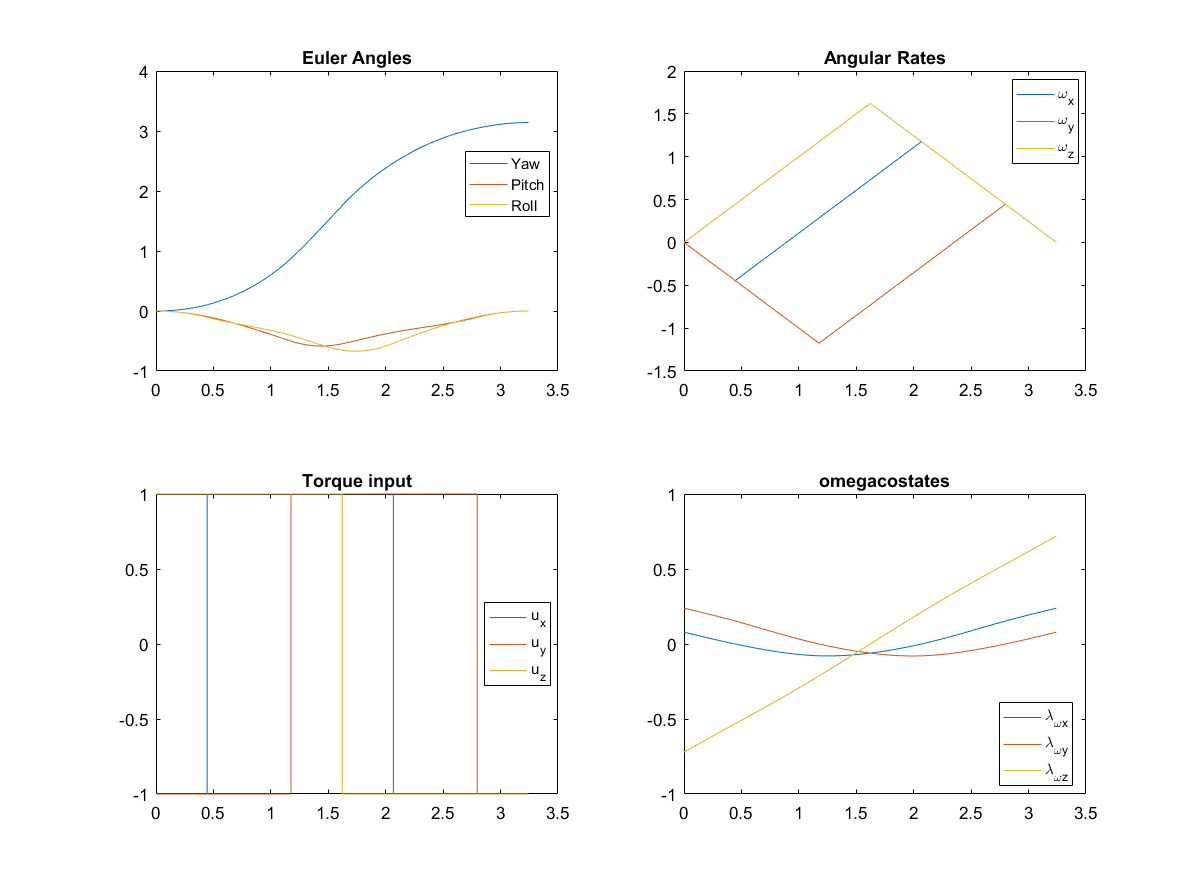
\includegraphics[height=12cm,keepaspectratio]{media/BilimorialInftyManeuver.png}
	\caption{180 yaw degree maneuver. Reproduced from Bilimoria\cite{bilimoria1993time}}
	\label{fig:bilimoriaResults}
\end{figure}

It is interesting to note that the maneuver time has decreased with respect to the eigenaxis maneuver even though we are following a longer path. This is because the controller is reorienting the body so that a torque greater than any individual limit is applied in the desired rotation of motion from an inertial perspective as pointed out by Bilimoria\cite{bilimoria1993time}.

